% arara: pdflatex
%Began 24 April 2025 --- 
\documentclass[a4paper,x11names,svgnames,10pt]{article}
\usepackage{amsmath}
\usepackage{hyperref}
% the \hypersetup{keyvals} commented out below is stored in an external hyperref.cfg file
% to enable the pagebackref=true option
%\hypersetup{%dvips, % not needed for  pdflatex
%	pagebackref=true,
%	pdfauthor={Iam The Author},
%	hyperfigures,
%	bookmarks=true,
%	bookmarksnumbered=true,
%	bookmarksopen=true,
%	colorlinks=true, %if true, link borders absent
%	pdfborder={1 1 1},
%	citecolor=blue,
%	linkcolor=blue,
%	urlcolor=blue,
%}
\usepackage{url}
\usepackage{svg}
\usepackage[utf8]{inputenc}
\usepackage{graphicx}
\usepackage{xcolor}
\usepackage{float}
\usepackage{natbib}

\topmargin -0.50in
\oddsidemargin 0.0in
\textwidth 6.27in
\textheight 9.75in

%%%-----------------------------------------------------
%%% TO BE EDITED FOR EACH NEW SERIES or VOLUME GENERATED 
%%%-----------------------------------------------------
	\def\authorName{I Am The Author}
	\def\authorFirstMidNameInit{I.\ T.\ }
	\def\authorLastName{Author}
	\def\dateGenerated{\today}
	\def\volNumber{I}
	\def\mdgBookTitle{Musical Dice Game - \\[0.15cm] Minuets and Trios \volNumber}
	\def\mdgBookSubTitle{{\small based on}\\ Musicalische Cabala \\[0.15cm] by Franciscus Schola (1773)  }
	\def\theBookSeries{Wonders of the Musical World Series 10}
	\def\theBookPublisher{Libre Edition Press}
	\def\theBookPublisherLogo{../images/1ed.png}
	\def\theBookFrontCover{../images/FrontCover.pdf}
%%%-----------------------------------------------------
%%%

\def\uline{\underline}
%\definecolor{orange}{rgb}{1,0.5,0} % RGB
%\definecolor{light-gray}{gray}{0.95} % shades
%\definecolor{orange}{cmyk}{0,0.5,1,0} % CMYK

\newcommand{\HRule}{\rule{\linewidth}{0.5mm}}

\setlength{\parindent}{0pt}

\DeclareGraphicsExtensions{.pdf,.png}

\setcitestyle{authoryear,round,comma,aysep={,},yysep={,},notesep={, }}

\title{\textsc{\mdgBookTitle}}
\author{\textsc{\authorFirstMidNameInit \authorLastName}}
\date{\textsc{\dateGenerated}}
% ---

\begin{document}
	
% Book Cover
% File name: mdgBooSVG10v1-cover.tex
% Purpose: Book Cover
% Instruction: Should be \input{.} just after \begin{document}
{
\topmargin 0.00in
\oddsidemargin 0.45in
\textwidth 8.50in
\textheight 11.50in
\thispagestyle{empty}

\begin{titlepage}

\begin{picture}(0,0)%
\linethickness{67.00pt}
\color{blue!22!black}
\put(-105,85){\line(1,0){6477}}
\put(-105,-699){\includegraphics[clip=true,trim=0.0in 0.45in 0.00in 1.5in, height=11.5in,width=8.80in,keepaspectratio]%
	{\theBookFrontCover}}
\put(-105,-692){\line(1,0){6477}}
\end{picture}

\vspace{-1.50in}

\begin{center}
	\LARGE\textbf{\color{white} \theBookSeries}
\end{center}

\vspace{-0.25in}
\vspace*{2.\baselineskip}
\begin{center} \Huge\textbf{\color{DarkBlue!40!DarkBlue}\em \mdgBookTitle}
\end{center}

\begin{center}
	\Large\textbf{\color{DarkBlue!40!DarkBlue}\em \mdgBookSubTitle}
\end{center}

\begin{center}
	\LARGE\textbf{\color{DarkBlue!20!DarkBlue}\em compiled by \authorFirstMidNameInit \authorLastName}
\end{center}

\vfill
\begin{center}
	\LARGE\textbf{\color{white}\em \theBookPublisher \\ \vspace{-0.25in}}
\end{center}
\end{titlepage}
}




\newpage
% Title Page
{
${}_{}$\\
\vspace{1.00in}	
\thispagestyle{empty}
\begin{center}
	\HRule \\[0.4cm]
	{\huge \bfseries \mdgBookTitle} \\[0.2cm]
	{\large{\em \mdgBookSubTitle} }\\[0.2cm]
	\HRule \\[1.5cm]
	% Author and supervisor
	\begin{minipage}{0.4\textwidth}
		\begin{flushleft} \large
			\emph{Author:}\\
			\authorFirstMidNameInit \textsc{\authorLastName}
		\end{flushleft}
	\end{minipage}
	\begin{minipage}{0.4\textwidth}
		\begin{flushright} \large
			\emph{Supervisor:} \\
			Dr. Communio \textsc{Sanctorum}
		\end{flushright}
	\end{minipage}
	\vfill
	% Bottom of the page
	{\textsc{\Large \theBookSeries}}  \\[0.2cm] 
	\includegraphics*[width=0.15\linewidth]{\theBookPublisherLogo}\\ 
	{\large \theBookPublisher \\
		\dateGenerated }\\
	\vspace{2.50in}
\end{center}
\newpage

%\maketitle		% uncomment if no Front Cover

\tableofcontents\label{tabofcon}

%\extrafloats{182}

\baselineskip 14pt

\newpage
\section[Introduction]{Introduction\footnote{The information contained in the introduction were culled from the following online resources:
		\citet{schola1773},
		\citet{wiki_mw2017},
		\url{https://opus-infinity.org/}, and 
		\href{https://www.sciencenews.org/article/mozarts-melody-machine-0}{Mozart's Melody Machine} \citep*{peterson2001}
	}
}
\begin{center}
	\begin{minipage}{0.4\textwidth}
		\begin{flushleft}
			\begin{center}
				``\small Musicalishe Cabala \\ Vermitelst welcher man \\ à Tre auf ein Travers. Violin. und Basso \\ wie auch Menuets und Tria Vor das Clavicen \\ mit einem eintzigen würfel-Spiehl, \\ ohne aller mihe und Khopfbrechen \\ zu Componieren Vermag. \\ Erfunden Von mir \\ Francesu Schola Chirurgu. \\ d.\ 10: Augustÿ 1773."
			\end{center}
		\end{flushleft}
	\end{minipage}
	\begin{minipage}{0.4\textwidth}
		\begin{flushright}
			\begin{center}
				``\small Musical Cabala \\ showing a method by which one, \\ for three: a flute, violin, and basso, \\ as well as minuets and trio for the clavier, \\ with a single die, \\ without any effort and headache, \\ to compose. \\
				Discovered by me \\ Francesu Schola Surgeon \\ d.\ 10: August 1773."
			\end{center}
		\end{flushright}
	\end{minipage}
\end{center}

Thus run the German title and corresponding English translation of the Musical Dice Game (MDG) that was authored by Franciscus Schola in 1773 (\citealp{schola1773}).  Rightly and interestingly so, as the Rules provided in this work allow a non-professional musician to generate (``compose") nearly 17.3 decillions ($17.3 \times 10^{33}$) of MDG minuet-trios.  More precisely, the total number of minuet-trios that the rules of the \href{https://imslp.org/wiki/Musicalische_Cabala_(Schola%2C_Franciscus)}{{\em Musicalische Cabala}}, as we would refer to this MDG from here onward, yield is: $$6^{44} = 17,324,272,922,341,479,351,919,144,385,642,496.$$

\noindent A {\it Musikalisches W\"{u}rfelspiel} (German for ``musical dice game" or MDG) is a system for randomly ``generating" (e.g., by using a die or two dice) musical compositions from precomposed options and was quite popular throughout Western Europe in the 18th century.  The earliest known MDG is Johann Philipp Kirnberger's {\em Der allezeit fertige Polonoisen- und Menuettencomponist (1st ed.\ 1757; rev.\ 2nd ed.\ 1783)} (translated from German as ``The Ever-Ready Minuet and Polonaise Composer").  Other well-known composers that are to known to have composed a MDG are C.P.E.\ Bach ({\em Einfall, einen doppelten Contrapunct in der Octave von sechs Tacten zu machen, ohne die Regeln davon zu wissen (1758)}; translated from German as ``A method for making six bars of double counterpoint at the octave without knowing the rules"), Abb\'{e} Maximillian Stadler ({\em Table pour composer des minuets et des Trios \`{a} la infinie; avec deux dez \`{a} jouer (1780)}; translated from French as ``A table for composing minuets and trios to infinity, by playing with two dice"), the latter MDG being also attributed to Franz Joseph Haydn.\\

Probably the most famous of MDGs is {\it Musikalisches W\"{u}rfelspiel K. 516f (1787)}.  This MDG was first published by J.J. Hummel in 1793 in Berlin and was republished in 1796 by Nikolaus Simrock in Bonn (as K. 294d or K. Anh. C 30.01). Simrock attributed this work to Wolfgang Amadeus Mozart. It is also known under the title of {\em Anleitung zum Componieren von Walzern so viele man will vermittelst zweier W\"{u}rfel, ohne etwas von der Musik oder Composition zu verstehen} (German for ``Instructions for the composition of as many waltzes as one desires with two dice, without understanding anything about music or composition") and may have been based on Mozart's manuscript {\em K.\ 516f}, written in 1787, consisting of numerous two-bar fragments of music, that appear to be some kind of game or system for constructing music out of two-bar fragments, but contains no instructions nor hints as to the use of dice.  An \href{(http://www.asahi-net.or.jp/\~rb5h-ngc/e/k516f.htm}{online article} by Hideo Noguchi offers a possible explanation for this attribution.\\

For this book, we generate MDG minuet-trios based on the rules given in \href{https://imslp.org/wiki/Musicalische_Cabala_(Schola\%2C_Franciscus)}{{\em Musicalische Cabala}}. Twenty (20) such MDG minuet-trios are given toward the latter part of this book. The scores of these generated minuet-trios were initially written using the \texttt{abc} environment of Chris Walshaw, then converted to Scalar Vector Graphics (SVG) images (with corresponding MIDIs) using {\tt abcm2ps} and {\tt abcmidi}, and then pre-processed with Inkscape to be included in \LaTeX\ to produce this book.


\section{\em Musicalische Cabala}

\subsection{Rules}\label{mdgRules}

The Rules provided in \href{https://imslp.org/wiki/Musicalische_Cabala_(Schola\%2C_Franciscus)}{{\em Musicalische Cabala}} generate minuet-trios consisting of 44 bars/measures that may be divided into three main parts: a first part (Part I) of 12 bars and two additional parts (Parts II and III) of 16 bars each. Each of  Parts II and III are composed of an eight-bar minuet and an eight-bar trio.  Each part or sub-part is played with a repeat. All told, a total of $88 \times 2 \;=\; 44$ bars of music is expected to be played for each {\it Musicalische Cabala} minuet-trio. Parts I and II are composed for three instruments: a transverse flute, a violin, and a cello, while Part III is composed for a clavier (or harpsichord).\\

The notes for each bar of the minuet are determined by rolling an ordinary six-sided die 44 times to get a sequence of integers whose terms are elements of the set \{1, 2, 3, ,4, 5, 6\}. The first 12 toss outcomes will be used to create the eight bars of Part I of the minuet-trio, the next 16 tosses for Part II (eight tosses each for the minuet and trio), and the last 16 tosses for Part III (eight tosses for the minuet, likewise for the trio). The notes for each measure are then obtained by consulting the Cabalas (inserts between pages 4 and 5; pages 7 (Part I), 9 (Part II), and 11 (Part III) of the PDF) \href{https://imslp.org/wiki/Musicalische_Cabala_(Schola\%2C_Franciscus)}{{\em Musicalische Cabala}}. The bar numbers corresponding to dice roll outcomes from these three Cabalas are summarized in Table~\ref{tab:tabNum} below.

\addcontentsline{toc}{subsection}{\hspace*{0.25in} {\em Cabalas for Parts I, II and III}}	
\begin{table}[H]
	\centering
	\begin{tabular}{c}
		\centering
		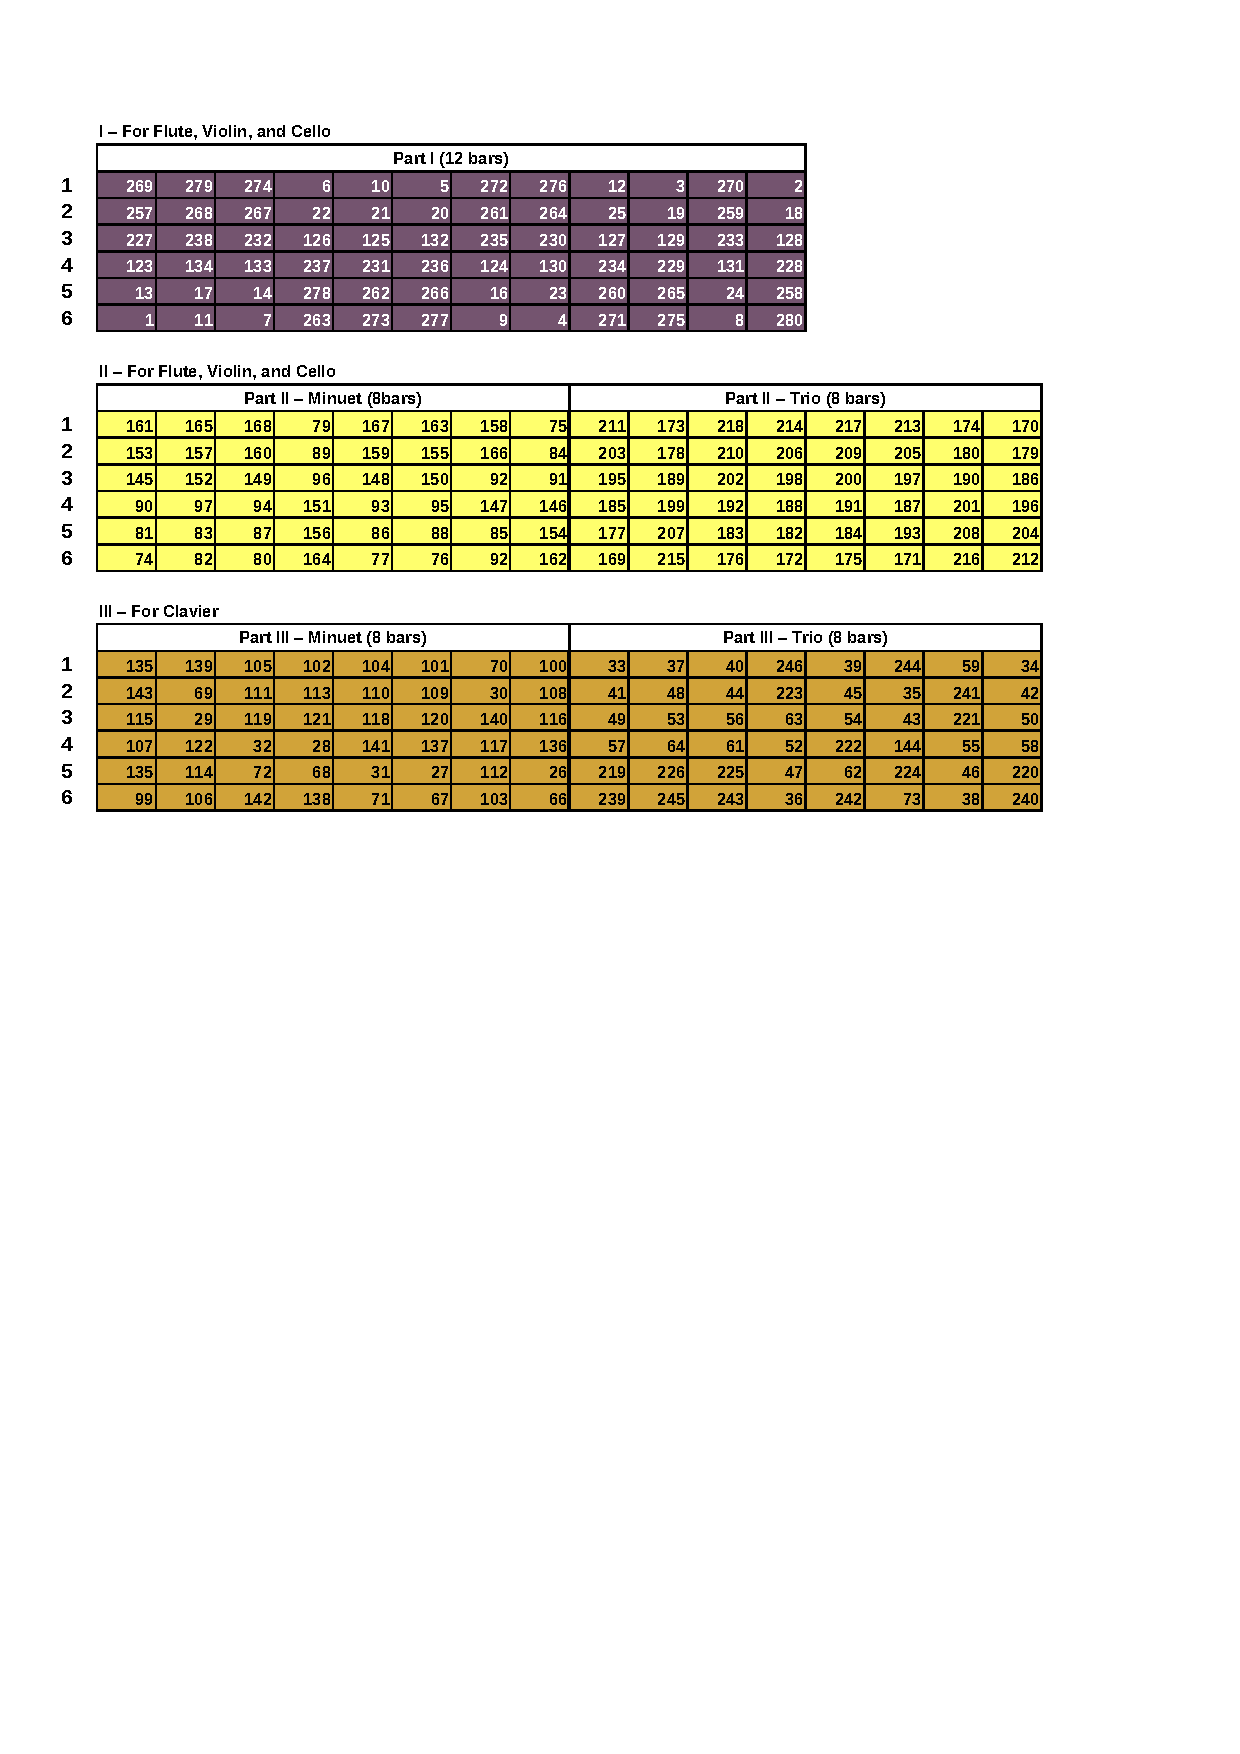
\includegraphics[clip=true,trim=0.275in 6.275in 1.00in 0.775in,scale=0.90]{000tables}
	\end{tabular}
	\caption{Table of bar numbers (from the Cabalas) to be used to determine the particular bar (numbered 1 to 280) to be looked up from the Table of Measures (Figures~\ref{fig:meas1} to \ref{fig:meas10}).}
	\label{tab:tabNum}
\end{table}

To obtain the notes to be played the particular bar of each part (Parts I, II, or III) of the minuet-trio to be constructed, simply look up the notes in the Table of Measures (Figures~\ref{fig:meas1} to \ref{fig:meas10}) for that bar number (numbered 1 to 280) obtained from the appropriate Cabala based on the die roll outcome.

For example, if we are in the process of creating the fifth bar (Bar 5) of Part I of the minuet and the dice outcome was a 3, then we would use the notes in bar number 125 of Figure~\ref{fig:meas5}: {\tt [V:1] {$^\wedge$d}e3/a/4c/4 b/a/g/f/} for the flute, {\tt [V:2] A3/c/4e/4 d/c/B/A/} for the violin, and {\tt [V:5] C,CDD,} for the cello.


\subsection{Table of Measures}\label{tabMeas}

The Table of Measures for Part I, II, and III of the minuet-trios based on \href{https://imslp.org/wiki/Musicalische_Cabala_(Schola\%2C_Franciscus)}{{\em Musicalische Cabala}} (noted for Set 1 only; there is a Set 2 also but it is not included here) are given in Figures~\ref{fig:meas1} to  \ref{fig:meas10} that follow. 

%\newpage
${}_{}$\\
%\vspace{0.10in}
\addcontentsline{toc}{subsection}{\hspace*{0.25in} {\em Musicalische Cabala - Set 1} of measures (page 1/10)}	
\begin{figure}[H]
	\centering
	\def\svgwidth{0.975\columnwidth}
 	\input{schola-1001.pdf_tex}
	\caption{Table of Measures - Set 1 (Page 1/10)}
	\label{fig:meas1}
\end{figure}

%\newpage
${}_{}$\\
\vspace*{0.5in}
\addcontentsline{toc}{subsection}{\hspace*{0.25in} {\em Musicalische Cabala - Set 1} of measures (page 2/10)}	
\begin{figure}[H]
	\centering
	\def\svgwidth{0.975\columnwidth}
 	\input{schola-1002.pdf_tex}
	\caption{Table of Measures - Set 1 (Page 2/10)}
	\label{fig:meas2}
\end{figure}

${}_{}$\\
\vspace*{0.5in}
\addcontentsline{toc}{subsection}{\hspace*{0.25in} {\em Musicalische Cabala - Set 1} of measures (page 3/10)}	
\begin{figure}[H]
	\centering
	\def\svgwidth{0.975\columnwidth}
 	\input{schola-1003.pdf_tex}
	\caption{Table of Measures - Set 1 (Page 3/10)}
	\label{fig:meas3}
\end{figure}

%\newpage
${}_{}$\\
\vspace*{0.5in}
\addcontentsline{toc}{subsection}{\hspace*{0.25in} {\em Musicalische Cabala - Set 1} of measures (page 4/10)}	
\begin{figure}[H]
	\centering
	\def\svgwidth{0.975\columnwidth}
 	\input{schola-1004.pdf_tex}
	\caption{Table of Measures - Set 1 (Page 4/10)}
	\label{fig:meas4}
\end{figure}

%\newpage
${}_{}$\\
\vspace*{0.5in}
\addcontentsline{toc}{subsection}{\hspace*{0.25in} {\em Musicalische Cabala - Set 1} of measures (page 5/10)}	
\begin{figure}[H]
	\centering
	\def\svgwidth{0.975\columnwidth}
	 	\input{schola-1005.pdf_tex}
	\caption{Table of Measures - Set 1 (Page 5/10)}
	\label{fig:meas5}
\end{figure}

%\newpage
${}_{}$\\
\vspace*{0.5in}
\addcontentsline{toc}{subsection}{\hspace*{0.25in} {\em Musicalische Cabala - Set 1} of measures (page 6/10)}	
\begin{figure}[H]
	\centering
	\def\svgwidth{0.975\columnwidth}
	 	\input{schola-1006.pdf_tex}
	\caption{Table of Measures - Set 1 (Page 6/10)}
	\label{fig:meas6}
\end{figure}

${}_{}$\\
\vspace*{0.5in}
\addcontentsline{toc}{subsection}{\hspace*{0.25in} {\em Musicalische Cabala - Set 1} of measures (page 7/10)}	
\begin{figure}[H]
	\centering
	\def\svgwidth{0.975\columnwidth}
	 	\input{schola-1007.pdf_tex}
	\caption{Table of Measures - Set 1 (Page 7/10)}
	\label{fig:meas7}
\end{figure}

%\newpage
${}_{}$\\
\vspace*{0.5in}
\addcontentsline{toc}{subsection}{\hspace*{0.25in} {\em Musicalische Cabala - Set 1} of measures (page 8/10)}	
\begin{figure}[H]
	\centering
	\def\svgwidth{0.975\columnwidth}
	 	\input{schola-1008.pdf_tex}
	\caption{Table of Measures - Set I (Page 8/10)}
	\label{fig:meas8}
\end{figure}

${}_{}$\\
\vspace*{0.5in}
\addcontentsline{toc}{subsection}{\hspace*{0.25in} {\em Musicalische Cabala - Set 1} of measures (page 9/10)}	
\begin{figure}[H]
	\centering
	\def\svgwidth{0.975\columnwidth}
	 	\input{schola-1009.pdf_tex}
	\caption{Table of Measures - Set 1 (Page 9/10)}
	\label{fig:meas9}
\end{figure}

%\newpage
${}_{}$\\
\vspace*{0.5in}
\addcontentsline{toc}{subsection}{\hspace*{0.25in} {\em Musicalische Cabala - Set 1} of measures (page 10/10)}	
\begin{figure}[H]
	\centering
	\def\svgwidth{0.975\columnwidth}
	 	\input{schola-1010.pdf_tex}
	\caption{Table of Measures - Set I (Page 10/10)}
	\label{fig:meas10}
\end{figure}


%\newpage
\section{Related Links}
The following are very interesting sites in that they allow the online rendering of MDGs:
\begin{itemize}
	\item \href{https://opus-infinity.org}{Opus Infinity} - Collaborative work of Robbert Harms, Hein Moors, and Suus van Petegem whose goal is to unravel the mystery behind the tables used for generating MDGs.  Site visitors can generate MDGs based on works of Kirnberger, Mozart, Stadler/Haydn, Bach, Gerlach, and Callegari ({\it 1st Cahier}).  Corresponding audio files ({\tt mid, ogg,} and/or {\tt mp3}) and image files ({\tt pdf} or {\tt png}) are also made available for listening, viewing, or downloading.
	
	\item  \href{http://sunsite.univie.ac.at/Mozart/dice/}{Mozart} - A site maintained by John Chuang that allows the site visitor to generate MDGs based on the work of Stadler/Haydn.
	
	\item  \href{https://marian-aldenhoevel.de/mozart/}{Mozart} - A site maintained by Marian Aldenh\"{o}vel allows the visitor to generate a MDG (user-specified or randomly-generated) and the corresponding audio ({\tt midi, wav}) and image files ({\tt pdf, png}) based on {\em Musikalisches W\"{u}rferspiel, K.\ 516f}.
	
	\item \href{https://www.amaranthpublishing.com/mozart.zip}{\tt mozart.zip} -  This is a Windows software ({\small\textcopyright} 1995 VisionSoft) by John Chuang and Stephen Goodwin that generates MDG based on input from user and is available for {\it free} from  \href{http://www.amaranthpublishing.com/MozartDiceGame.htm}{Amaranth Publishing}.  
	
	\item \href{(http://www.asahi-net.or.jp/\~rb5h-ngc/e/k516f.htm}{``Mozart - Musical Game in C K. 516f,"}	Mozart Studies Online - The site of Hideo Noguchi that offers an explanation linking {\em Musikalisches W\"{u}rferspiel, K.\ 516f}, and  {\em K.\ 294d (K.\ Anh.\ C 30.01)}. 
\end{itemize}

%\newpage
\section{Acknowledgments}
Special thanks to \href{https://imslp.org}{International Music Score Library Project} for \href{https://imslp.org/wiki/Ludus_Melothedicus_(Anonymous)}{\it Musicalische Cabala, ou Le Jeu de Dez Harmonique, 2nd ed. (1759)}, \href{https://opus-infinity.org}{Opus Infinity} for additional related information, and \href{http://www.amaranthpublishing.com/MozartDiceGame.htm}{Amaranth Publishing} for a copy of {\tt mozart.zip}. My sincerest gratitude to Chris Walshaw et al. for the \href{http://www.abcnotation.com/}{ABC music notation}; Jean-Francois Moine for \href{http://moinejf.free.fr/}{\tt abcm2ps} and the accompanying examples, templates, and pointers for the appropriate use of these resources; Guido Gonzato for the \href{http://abcplus.sourceforge.net/}{ABC Plus Project} and the \href{http://abcplus.sourceforge.net/#abcMIDI}{{\tt abcmidi} resources} available there, more especially for the ABC resource book {\em Making Music with ABC 2}; James R. Allwright and Seymour Shlien for \href{http://abc.sourceforge.net/abcMIDI}{\tt abcmidi} source and binaries; \href{https://artifex.com/}{Artifex, Inc.} for Ghostscript v.10.00.0 (includes the {\tt ps2pdf} converter); \href{https://www.inkscape.org/}{Inkscape v.1.2.2} for the tool for converting SVGs to PDFs for inclusion into \LaTeX\ documents; William Schelter for \href{https://maxima.sourceforge.io}{Maxima v.5.47.0}---used for computing the permutation number; \href{https://google.lens}{Google Lens} and \href{https://translate.google.com}{Google Translate} for aiding in producing the English versions of the text of \href{https://imslp.org/wiki/Musicalische_Cabala_(Schola\%2C_Franciscus)}{{\em Musicalische Cabala}}; Colomban Wendling et.\ al for \href{https://www.geany.org}{Geany 2.0 IDE}; and \href{https://tex.stackexchange.com/users/632/martin-h}{\tt User:Martin H} for his \href{https://tex.stackexchange.com/questions/2099/how-to-include-svg-diagrams-in-latex}{reply} to a \TeX\ / \LaTeX\ Stack Exchange question on including SVGs into \LaTeX\ documents. Thanks to  Ditto to Machtelt Garrels for the book \href{http://tldp.org/LDP/Bash-Beginners-Guide/html/Bash-Beginners-Guide.html}{Bash Guide for Beginners}, Vivek Gite for the book \href{http://www.freeos.com/guides/lsst/}{Linux Script Shell Tutorial}, and Steve Parker for the \href{http://steve-parker.org/sh/cheatsheet.pdf}{Unix/Linux Shell Cheatsheet}. John Fogarty's GitHub Site: \href{https://github.com/jfogarty/latex-createspace-bookcover}{Latex CreateSpace BookCover} and Peter Wilson's reply in  \TeX\ / \LaTeX\ Stack Exchange on \href{https://tex.stackexchange.com/questions/17579/how-can-i-design-a-book-cover}{designing a book cover}, were sources of ideas, information, and materials for creating the book cover and title page, thanks to both of them; \href{http://www.libreoffice.org/}{LibreOffice Calc} for its use in the image creation of the book cover.  Many thanks, too, to the \href{https://www.debian.org}{Debian Project} for the Debian 12 (Bookworm) GNU/Linux OS, \href{http://www.tug.org/texlive/}{TeXLive} for providing the \TeX\ distribution,  and \href{https://github.com}{GitHub} for its generosity in providing space for \href{https://github.com/justineuro/mdgBookSVG8Kit}{the project}.  

\newpage
\section{Twenty (20) Selected Minuets based on \href{https://imslp.org/wiki/Musicalische_Cabala_(Schola\%2C_Franciscus)}{{\em Musicalische Cabala}}}
%\vspace{-.10in}
This section contains an example of twenty (20) minuet-trios that were generated using the Rules in Section~\ref{mdgRules}. 
\vspace{0.20in}
{
	\topmargin -0.25in
	\textheight 9.25in
	\input{svgList}
}	

%\newpage
\vspace{0.25in}
\section{License}
This work by I Am The Author, based on work of J.L.A. Uro at \url{https://github.com/justineuro/mdgBookSVG10Kit}, is licensed under a Creative Commons Public Domain International License.

\bibliographystyle{plainnat}
\bibliography{mdg10}



\end{document}
